\section{Vergelijkingsoverzicht}
\label{sec:evaluatie-spinnenweb}

Figuur \ref{fig:spinnenweb-final} toont een overzicht van de scores van de vier raamwerken op de vijf criteria in de vorm van een spinnenweb.
De formules van de vergelijkingscriteria voor het plotten van het spinnenweb kunnen teruggevonden worden in sectie \ref{sec:vergelijking-spinnenweb}.
Daar werden de gerelativeerde formules voorgesteld om een score tussen $0$ en $1$ te bekomen.
Ook werden de formules voor productiviteit en performantie geïnverteerd omdat voor deze criteria geldt:  hoe lager de score, hoe beter het raamwerk.

\begin{figure}
  \centering
  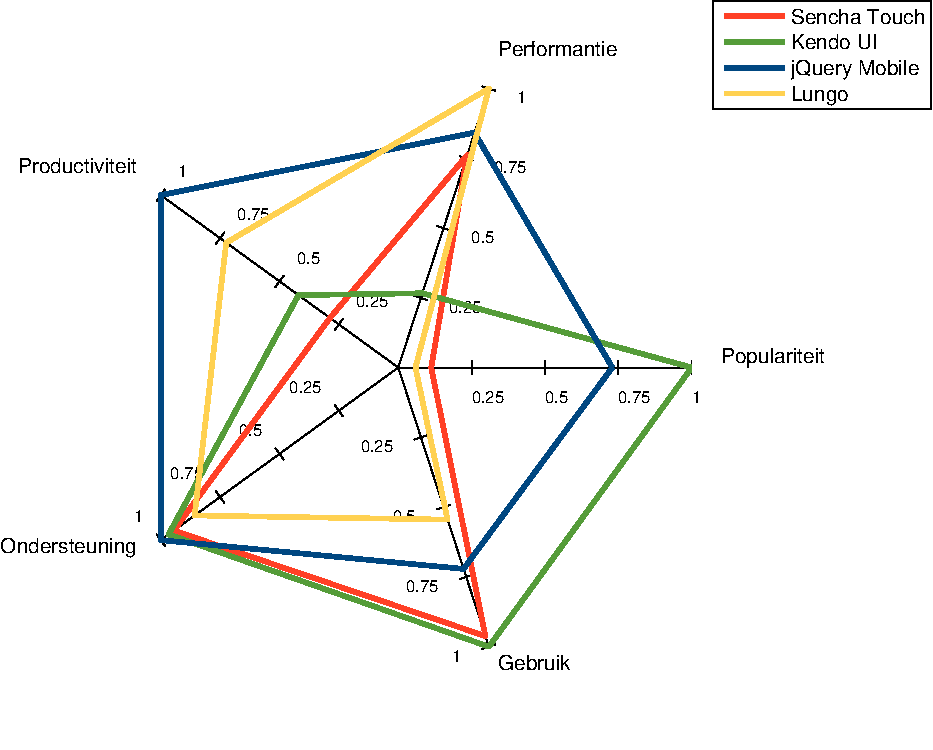
\includegraphics[width=\textwidth]{figuren/spidergraph-final-nl.pdf}
  \caption{Vergelijkingsoverzicht met de vijf vergelijkingscriteria voor \st{},  \kendo{},  \jqm{} en \lungo{}.}
  \label{fig:spinnenweb-final}
\end{figure}

De formules van de vergelijkingscriteria voor het plotten van het spinnenweb kunnen teruggevonden worden in sectie \ref{sec:vergelijking-spinnenweb}.
Daar werden de gerelativeerde formules voorgesteld om een score tussen $0$ en $1$ te bekomen.
Ook werden de formules voor productiviteit en performantie geinverteerd omdat voor deze criteria geldt:  hoe lager de score, hoe beter het raamwerk.

De formules van productiviteit en performantie zijn echter gewijzigd na de evaluatie en werden formule \ref{eq:productiviteit-enhanced} en \ref{eq:performantie-enhanced}.
Hun nieuwe relatieve formules zijn dan respectievelijk

\begin{equation}
  \text{Productiviteit}_r^{\pentagon} = \frac{\text{Productiviteit}_r^{'-1}}{\underset{m}{\max}\{\text{Productiviteit}_m^{'-1}\}}
  \label{eq:rel-productiviteit-2}
\end{equation}

en

\begin{equation}
  \text{Performantie}_r^{\pentagon}= \frac{\text{Performantie}_r^{'-1}}{\underset{m}{\max}\{\text{Performantie}_m^{'-1}\}}
  \label{eq:rel-performantie-2}
\end{equation}

% De oppervlakten van de vier vijfhoeken is de volgende:
% \begin{description}
% %nieuwste data
%  \item [\jqm{}] $1.76$
%  \item [\kendo{}] $1.31$
%  \item [\lungo{}] $0.90$
%  \item [\st{}] $0.76$
% \end{description}


In wat volgt zullen de raamwerken besproken worden, door de oppervlaktes van vijhoeken te bekijken en conclusies te trekken over de resultaten van alle criteria.
De eenheid van de oppervlaktes komt overeen met de eenheid zoals weergegeven op de assen van het spinnenweb.

% but...

\jqm{} heeft de grootste oppervlakte ($1.76$) en is de winnaar.
Een van de belangrijkste factoren die \jqm{} tot winnaar maakt is het feit dat er geen architectuur wordt afgedwongen.
Dit maakt dat de leercurve veel lager ligt ten voordele van de productiviteit.
Ook een betere documentatie en omkadering maakt \jqm{} productiever.
De grotere populariteit in vergelijking met \lungo{} maakt \jqm{} aantrekkelijker als er geen architectuur noodzakelijk is.
De afwezigheid van een architectuur brengt echter twee nadelen met zich mee.
Ten eerst zal het raamwerk minder functionaliteit kunnen aanbieden.
Door plug-ins en HTML5-kenmerken zal dit gebrek aan functionaliteit toch beperkt blijven.
Een tweede nadeel is de code die moet geschreven worden bij gebruik van het \jqm{} raamwerk.
\jqm{} is opmaakgedreven waarbij veel HTML-code moet worden geschreven met grote verbositeit.
Dit maakt het linken van HTML- met \js{}-code foutgevoelig.

% jQM volgt % Waarom kiezen voor jqm:
% +/- geen architectuur (
    % minder gebruik
    % lagere leercurve (veel HTML, link met js is het lastigst)
    % meer code schrijven (error prone)
% + zeer populair (jQuery core) zie stackoverlow => vragen worden door een hele community opgelost (geen payed support)
% als een easy (geen architectuur) raamwerk + populair (belangrijke klanten,  gekend op social media)

\kendo{} bekleedt de tweede plaats met een opervlakte van $1.31$.
In tegenstelling tot \jqm{} heeft het wel een architectuur en is het dus meer bruikbaar.
De score van de productiviteit bevindt zich onder de helft maar in vergelijking met \st{} scoort het beter.
Het grote nadeel van \kendo{},  wat niet in het spinnenweb kan worden gezien,  is de hoge kost voor een licentie.
Het feit dat \kendo{} niet \term{open-source} is reflecteerd zich echter niet in de populariteit.
Van alle vier raamwerken is \kendo{} het minst performant.
De downloadtijden waren lager in vergelijking met \st{} maar de crashes op iOS-toestellen zorgden voor een lage gebruikservaring.
Het feit dat \kendo{} een \term{native look-and-feel} aanbiedt is een belangrijk kenmerk maar dit kan ook niet op het spinnenweb worden teruggevonden.
De iOS-lay-out is sterk gelijkend is op de echte iOS-lay-out.
Dit was bij Android minder geslaagd.

% kendo is winnaar (uitstekend op pop, gebruik en ondersteuning % Waarom kiezen voor kendo:
% - architectuur => minder productief maar meer bruikbaar
% - hoge licentiekost => professionele support. Ondanks niet open source toch populiar (meest populair)
% + native look-and-feel => downloadtijden stijgen?  meer op native applicatie (positieve impact niet geevalueerd) (iOS lay-out sterk gelijkend op
%echte iOS,  Android minder gelijkend, Blackberry en windows niet bekeken)

\lungo{} heeft de derde grootste oppervlakte ($0.90$).
Op drie van de vijf criteria scoort \lungo{} het slechtst.
Er is geen architectuur opgelegd en weer kan dit voor- en nadeel zowel in productiviteit en gebruik opgemerkt worden.
De voordelen bij productiviteit zijn echter minder dan \jqm{} omdat de ondersteuning en documentatie minimaal is.
De nadelen bij gebruik zijn dan weer uitvergroot omdat er niet zoveel functionaliteit en plug-ins als bij \jqm{} konden werden teruggevonden.
Positief is dan weer dat \lungo{} de beste downloadtijden behaalden omdat \quo{}, de \js{}-bibliotheek van \lungo{},  geoptimaliseerd is voor mobiele apparaten.
De testen op gebruikservaring zwakte de performantie van \lungo{} af.
\lungo{} is veruit het minst populair.
Dit kan zowel met de literatuur als met sociale netwerken bevestigd worden.

% tweede is lungo % Waarom kiezen voor lungo:
% - productiviteit => verkeerde indruk (zonder voorkennis / sumire documentatie maakt het moeilijk)
% - support => niet bij oudere android OS (2.3) X)(marktwaarde android 2.3 tov alle devices)X% van de devices vallen dan uit de boot
% + performatie zeer positief => quo js geoptimaliseerd (bedrijf gespecialiseerd in mobile user experience)! (weinig support help hier ook)
% nauwelijks bekend (literatuur, social networks (zie populariteit), ...)

\st{} is volgens de gekozen criteria het slechtste raamwerk ($0.75$).
De combinatie van de MVC-architectuur en \js-gedreven opmaak maken \st{} zowel het minst productief als minst performant in vergelijking met de andere raamwerken.
Alle HTML-code wordt door het raamwerk zelf aangemaakt waardoor de \js-bestanden zeer groot zijn.
De downloadtijden waren dan ook opmerkelijk langer door het Delta Update mechanisme
De gebruikservaringtesten gaven echter het tegenovergestelde resultaat want na de initiële wachttijd had \st{} de laagste responstijden.
De tools die Sencha aanbiedt om ontwikkelaars te helpen (Sencha Architect en Sencha Cmd) blijken niet voldoende om het verschil met andere raamwerken te dichten.
De tools laten werken is een leerproces op zich.
Hoewel de ondersteuning van \st{} hoog is, moet er opgemerkt worden dat het afhankelijk is van de WebKit \term{engine}.
Toestellen met een standaard browser die deze \term{engine} niet bevatten, zoals Windows Phone,  kunnen \st{} niet gebruiken.

% Sencha (nergens numero uno) % Waar niet kiezen voor st:
% + / - Tools voorhanden (Sencha Cmd / Architect ) om programmeren makkelijker te maken maar tools niet even handig (of betalend)
% - Javascript driven maakt het lastig (alle simple HTML moet in js worden geschreven): meeste lijnen JS + grote bibliotheek => minder performant
% - gebaseerd op webkit => geteste toestellen hadden dit wel (windows phone geen webkit)


%%%%%%%%%%%%%%%%% NIET BESPROKEN

% besluiten  (de getallen zijn geen procenten)
% 1) Kendo: 1,51 
% 2) Lungo: 1,14
% 3) jQM: 1,03
% 4) ST: 0,62

%%%%%%%%%%%%%%%%%%%%%%%%%%


% daarna de bindparagraaf door onze 2 improvents (productiviteit en performantie)
% referen naar de nieuwe formules in de respectievelijke secties
% nieuwe formules voor het bereken van het relatieve waarden voor de respectievelijke formules
% tonen van de finale grafiek


%nieuwe zaken finaal versus initieel:
%Productiviteit
  % jqm naar eerste plaats,  andere boeten in (raamwerk met architectuur komen achteraan,  stemt overeen met verwachtingen)
%Performantie:
  %Kendo: iOS crash van lange lijst: performantie daalt van 40% naar 25%
  %Sencha : Performantie verhoogt want gebruikservaring maximaal

%jQM naar eerst plaats, rest schuift een plaats door (buiten st)
% snelle ontwikkeling die performant is en overal ondersteund wordt geen payed support nodig hebt en geen geavanceerde features wil implementeren




